%% BioMed_Central_Tex_Template_v1.06
%%                                      %
%  bmc_article.tex            ver: 1.06 %
%                                       %

%%IMPORTANT: do not delete the first line of this template
%%It must be present to enable the BMC Submission system to
%%recognise this template!!

%%% additional documentclass options:
%  [doublespacing]
%  [linenumbers]   - put the line numbers on margins

\documentclass[twocolumn]{bmcart}
%\documentclass{bmcart}

%%% Load packages
%\usepackage{amsthm}
%\RequirePackage{natbib}
%\RequirePackage[authoryear]{natbib}% uncomment this for author-year bibliography
\usepackage{hyperref}
\usepackage[utf8]{inputenc} %unicode support
%\usepackage[applemac]{inputenc} %applemac support if unicode package fails
%\usepackage[latin1]{inputenc} %UNIX support if unicode package fails

\usepackage{graphicx}
\usepackage{minted}
\usemintedstyle{vs}

\usepackage{amsmath,amssymb}
\usepackage{booktabs}


%%%%%%%%%%%%%%%%%%%%%%%%%%%%%%%%%%%%%%%%%%%%%%%%%
%%                                             %%
%%  If you wish to display your graphics for   %%
%%  your own use using includegraphic or       %%
%%  includegraphics, then comment out the      %%
%%  following two lines of code.               %%
%%  NB: These line *must* be included when     %%
%%  submitting to BMC.                         %%
%%  All figure files must be submitted as      %%
%%  separate graphics through the BMC          %%
%%  submission process, not included in the    %%
%%  submitted article.                         %%
%%                                             %%
%%%%%%%%%%%%%%%%%%%%%%%%%%%%%%%%%%%%%%%%%%%%%%%%%


%\def\includegraphic{}
%\def\includegraphics{}

%%% Put your definitions there:
\startlocaldefs
\newcommand{\opentsne}{\textsf{openTSNE}}
\endlocaldefs

\begin{document}

%%% Start of article front matter
\begin{frontmatter}

\begin{fmbox}
\dochead{Software}

\title{openTSNE: a modular Python library for t-SNE dimensionality reduction and embedding}

%%%%%%%%%%%%%%%%%%%%%%%%%%%%%%%%%%%%%%%%%%%%%%
%%                                          %%
%% Enter the authors here                   %%
%%                                          %%
%% Specify information, if available,       %%
%% in the form:                             %%
%%   <key>={<id1>,<id2>}                    %%
%%   <key>=                                 %%
%% Comment or delete the keys which are     %%
%% not used. Repeat \author command as much %%
%% as required.                             %%
%%                                          %%
%%%%%%%%%%%%%%%%%%%%%%%%%%%%%%%%%%%%%%%%%%%%%%

\author[
   addressref={aff1},                   % id's of addresses, e.g. {aff1,aff2}
   corref={aff1},                       % id of corresponding address, if any
   %noteref={n1},                        % id's of article notes, if any
   email={pavlin.policar@fri.uni-lj.si}   % email address
]{\inits{PGP}\fnm{Pavlin G.} \snm{Poli\v{c}ar}}
\author[
   addressref={aff1,aff2}
]{\inits{MS}\fnm{Martin} \snm{Stra\v{z}ar}}
\author[
   addressref={aff1,aff3}
]{\inits{BZ}\fnm{Bla\v{z}} \snm{Zupan}}

%%%%%%%%%%%%%%%%%%%%%%%%%%%%%%%%%%%%%%%%%%%%%%
%%                                          %%
%% Enter the authors' addresses here        %%
%%                                          %%
%% Repeat \address commands as much as      %%
%% required.                                %%
%%                                          %%
%%%%%%%%%%%%%%%%%%%%%%%%%%%%%%%%%%%%%%%%%%%%%%

\address[id=aff1]{%
  \orgname{Faculty of Computer and Information Science, University of Ljubljana},
  %\street{Ve\v{c}na Pot 113},
  \postcode{SI 1000}
  \city{Ljubljana},
  \cny{Slovenia}
}
\address[id=aff2]{%
  \orgname{Broad Institute of Harvard and MIT},
  %\street{D\"{u}sternbrooker Weg 20},
  \postcode{MA 02142}
  \city{Cambridge},
  \cny{U.S.A.}
}
\address[id=aff3]{%
  \orgname{Department of Molecular and Human Genetics, Baylor College of Medicine},
  %\street{D\"{u}sternbrooker Weg 20},
  \postcode{TX 77030}
  \city{Houston},
  \cny{U.S.A.}
}

%%%%%%%%%%%%%%%%%%%%%%%%%%%%%%%%%%%%%%%%%%%%%%
%%                                          %%
%% Enter short notes here                   %%
%%                                          %%
%% Short notes will be after addresses      %%
%% on first page.                           %%
%%                                          %%
%%%%%%%%%%%%%%%%%%%%%%%%%%%%%%%%%%%%%%%%%%%%%%

%\begin{artnotes}
%\note{Sample of title note}     % note to the article
%\note[id=n1]{Equal contributor} % note, connected to author
%\end{artnotes}

\end{fmbox}% comment this for two column layout

%%%%%%%%%%%%%%%%%%%%%%%%%%%%%%%%%%%%%%%%%%%%%%
%%                                          %%
%% The Abstract begins here                 %%
%%                                          %%
%% Please refer to the Instructions for     %%
%% authors on http://www.biomedcentral.com  %%
%% and include the section headings         %%
%% accordingly for your article type.       %%
%%                                          %%
%%%%%%%%%%%%%%%%%%%%%%%%%%%%%%%%%%%%%%%%%%%%%%

\begin{abstractbox}

\begin{abstract}
Point-based visualisations of large, multi-dimensional data from molecular biology can reveal meaningful clusters. One of the most popular techniques to construct such visualisations is t-distributed stochastic neighbor embedding (t-SNE), for which a number of extensions have recently been proposed to address issues of scalability and the quality of the resulting visualisations. We introduce \opentsne, a modular Python library that implements the core t-SNE algorithm and its extensions. The library is orders of magnitude faster than existing popular implementations, including those from scikit-learn. Unique to \opentsne\ is also the mapping of new data to existing embeddings, which can surprisingly assist in solving batch effects.
\end{abstract}

%%%%%%%%%%%%%%%%%%%%%%%%%%%%%%%%%%%%%%%%%%%%%%
%%                                          %%
%% The keywords begin here                  %%
%%                                          %%
%% Put each keyword in separate \kwd{}.     %%
%%                                          %%
%%%%%%%%%%%%%%%%%%%%%%%%%%%%%%%%%%%%%%%%%%%%%%

\begin{keyword}
\kwd{t-SNE}
\kwd{embedding}
\kwd{visualization}
\kwd{dimensionality reduction}
\end{keyword}

% MSC classifications codes, if any
%\begin{keyword}[class=AMS]
%\kwd[Primary ]{}
%\kwd{}
%\kwd[; secondary ]{}
%\end{keyword}

\end{abstractbox}
%
%\end{fmbox}% uncomment this for twcolumn layout

\end{frontmatter}

%%%%%%%%%%%%%%%%%%%%%%%%%%%%%%%%%%%%%%%%%%%%%%
%%                                          %%
%% The Main Body begins here                %%
%%                                          %%
%% Please refer to the instructions for     %%
%% authors on:                              %%
%% http://www.biomedcentral.com/info/authors%%
%% and include the section headings         %%
%% accordingly for your article type.       %%
%%                                          %%
%% See the Results and Discussion section   %%
%% for details on how to create sub-sections%%
%%                                          %%
%% use \cite{...} to cite references        %%
%%  \cite{koon} and                         %%
%%  \cite{oreg,khar,zvai,xjon,schn,pond}    %%
%%  \nocite{smith,marg,hunn,advi,koha,mouse}%%
%%                                          %%
%%%%%%%%%%%%%%%%%%%%%%%%%%%%%%%%%%%%%%%%%%%%%%

%%%%%%%%%%%%%%%%%%%%%%%%% start of article main body
% <put your article body there>

%%%%%%%%%%%%%%%%
%% Background %%
%%
\section*{Background}

The abundance of high-dimensional data sets in molecular biology calls for
techniques for dimensionality reduction, and in particular for methods that can
help in the construction of data visualizations. Popular approaches for
dimensionality reduction include principal component analysis (PCA), multidimensional
scaling, t-distributed stochastic
neighbor embedding (t-SNE)~\cite{maaten2008visualizing}, and uniform manifold approximation and
projections (UMAP)~\cite{2018arXivUMAP}. Among these, t-SNE lately received much
attention as it can address high volumes of data and reveal meaningful
clustering structure. Most of the recent reports on single-cell gene expression
data start with an overview of the cell landscape, where t-SNE embeds
high-dimensional expression profiles into a two-dimensional
space~\cite{macosko2015highly,cao2019single,tasic2018shared}.
Figs.~\ref{fig:macosko}.a and \ref{fig:macosko}.b are examples of two such
embeddings.

\begin{figure*}[htbp]
  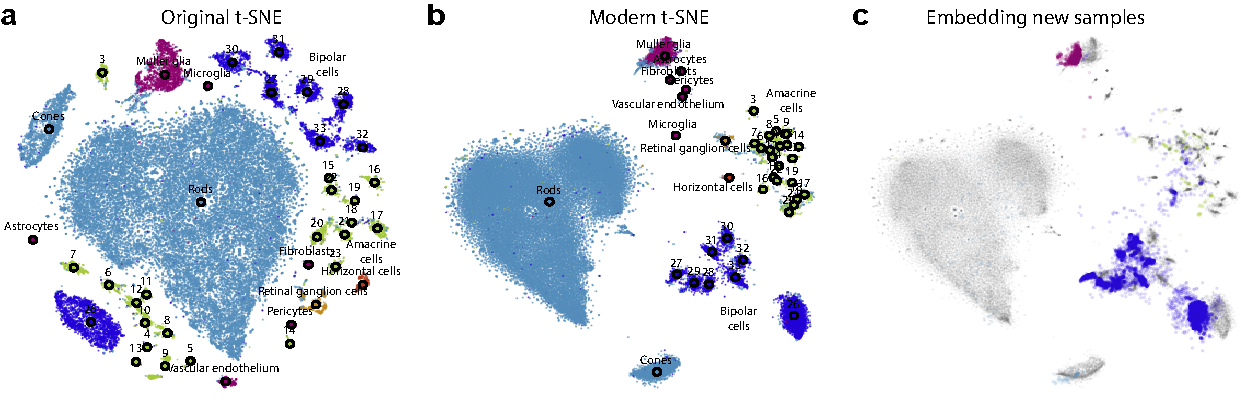
\includegraphics[width=\textwidth]{macosko2015}
  \caption{\label{fig:macosko}The figure shows the progression of t-SNE embeddings following theoretical advances, which are all included in \opentsne. The data in \textbf{(a)} and \textbf{(b)} represent 44,808 single-cell gene-expression profiles of mouse retinal cells from the study by Macosko \textit{et al.}~\cite{macosko2015highly}. Similarly, the data in \textbf{(c)} contains 27,499 expression profiles from mouse retinal cells from Shekhar \textit{et al.}~\cite{shekhar2016comprehensive}. \textbf{(a)} We construct a t-SNE embedding following the parameter choices from the original publication from Maaten \& Hinton~\cite{maaten2008visualizing}. The visualization shows poor preservation of the global organization of clusters, resulting from random initialization and an affinity model focused on preserving local neighborhoods. \textbf{(b)} shows a modern t-SNE embedding, utilizing the latest theoretical advances and practical recommendations. The embedding is constructed using a multi-scale affinity model, preserving both short-range and long-range interactions between data points, and is initialized such that the global layout is meaningful. Unlike in \textbf{(a)}, the green and blue clusters representing different sub-types of amacrine and bipolar cells are now localized to the same regions of the space, indicating a higher level of similarity than to other cell types. \textbf{(c)} shows how existing t-SNE reference atlases can be used to embed new samples into existing embeddings. The positions of new data points correspond to cell types from the reference atlas.}
\end{figure*}

Despite its utility, t-SNE has often been criticized for poor scalability when
addressing large data sets, lack of global organization -- t-SNE focuses on local
clusters that are arbitrarily scattered in the low-dimensional space -- and the
absence of theoretically-founded implementations to map new data into existing
embeddings~\cite{ding2018interpretable,becht2019dimensionality}. Most of these
shortcomings have recently been addressed. Linderman \textit{et
al.} sped-up the method through an interpolation-based
approximation, reducing the time complexity to be merely linear dependent on
the number of samples~\cite{linderman2019fast}. Kobak \& Berens proposed
several techniques to improve global positioning, including estimating
similarities with a mixture of Gaussian kernels~\cite{kobak2019art}. In our previous work, we presented
a principled approach for embedding new samples into existing visualizations~\cite{policar2019embedding}.


\section*{Results}

We introduce \opentsne, a comprehensive Python library that implements t-SNE and all its recently proposed extensions. Most notable among these are
\begin{enumerate}
\item the implementation of efficient approximation schemes~\cite{van2014accelerating,linderman2019fast} allowing the embedding of millions of data points,
\item the addition of new samples into existing embeddings~\cite{policar2019embedding},
\item better initialization schemes~\cite{kobak2019umap} leading to more globally consistent layouts,
\item variable degrees of freedom~\cite{kobak2019heavy} allowing the inspection of data at different levels of resolution,
\item multiscale similarity kernels~\cite{kobak2019art} which preserves small, well-defined clusters and uncovers global relationships between clusters, and
\item improved defaults for learning rate and the number of iterations~\cite{belkina2019automated} which produce embeddings at a lower computational cost.
\end{enumerate}

The library is fully compatible with the Python data-science ecosystem (e.g., \textsf{numpy}, \textsf{scikit-learn}, \textsf{scanpy}) providing a familiar and intuitive user interface to new users. Its modular design encourages extensibility and experimentation with various settings and changes in the analysis pipeline.

\opentsne\ is open-source and has become an integral part of the Python data science ecosystem. The package has received over 600 Github stars and has been downloaded hundreds of thousands of times, averaging in thousands of weekly downloads. The source code is publicly available on Github at \url{https://github.com/pavlin-policar/openTSNE}, and can be installed from \textsf{PyPI} and \textsf{conda-forge} -- the two most widely adopted Python package managers.

Accessibility is one of the core design principles of \opentsne. Our aim is to make the latest theoretical advances in t-SNE as accessible as possible to as many users as possible. As such, our API is based on the familiar \textsf{scikit-learn} interface~\cite{sklearn_api}, which enables users a smooth transition from existing Python libraries. For example, Fig.~\ref{fig:tasic} depicts four different t-SNE visualizations generated by \opentsne, each based on recent advances in the t-SNE algorithm. The code used to generate these embeddings is shown below.

\begin{minted}[
fontsize=\footnotesize,
frame=lines,
framesep=2mm,
baselinestretch=1.1
]{python}
import openTSNE
from openTSNE.affinity import Multiscale
# a - standard t-SNE
tsne1 = openTSNE.TSNE(perplexity=30).fit(X)
# b - high perplexity  for globa structure
tsne2 = openTSNE.TSNE(perplexity=500).fit(X)
# c - multiscale kernel for local/global structure
aff = Multiscale(X, perplexities=[30, 500])
tsne3 = openTSNE.TSNE(affinities=aff).fit(X)
# d - decrease dof for higher resolution
tsne4 = openTSNE.TSNE(dof=0.6).fit(X)
\end{minted}

\noindent The code snippet takes as input a \textsf{numpy} array or \textsf{scipy} sparse matrix \texttt{X} and produces four \texttt{TSNEEmbedding} objects. These may subsequently be subject to further optimization under different parameter settings or may be used to embed new samples into the embedding landscape. Additional parameters are omitted for clarity but can be found in accompanying notebooks publicly available at \url{https://github.com/pavlin-policar/opentsne-paper}.

\section*{Discussion}

\subsection*{Uncovering Structure in High-Dimensional Data}

Dimensionality reduction techniques implicitly assume that high-dimensional data lies on a lower-dimensional manifold, which can accurately be captured by a smaller number of dimensions. However, there is no evidence to suggest that any data set can accurately be described using only two dimensions and that any projection onto a two-dimensional plane will inevitably lead to loss of information. Therefore, it is beneficial to examine multiple embeddings, each of which provides a different perspective into the topology and other characteristics of the data.
\begin{figure*}[htbp]
  \includegraphics[width=\textwidth]{tasic2018}
  \caption{\label{fig:tasic}We use openTSNE to create four different visualizations of the Tasic \textit{et al.}~\cite{tasic2018shared} data set containing 21,874 single-cells originating from the mouse neocortex. Cluster annotations and colors are taken from the original publication. Warm colors correspond to excitatory neurons, cool colors correspond to inhibitory neurons, and gray/brown colors correspond to non-neuronal cells. The standard t-SNE \textbf{(a)} emphasizes local structure while increasing perplexity \textbf{(b)} results in a more meaningful layout of the clusters. We can also combine the two perplexities by using a multiscale kernel affinity model \textbf{(c)} and obtain a good trade-off between global and local structure. Alternatively, we can inspect more fine-grained structure and reveal smaller clusters by using a more heavy-tailed kernel \textbf{(d)}.}
\end{figure*}
For instance, in Fig.~\ref{fig:tasic}, we show four embeddings of the same gene-expression data from the mouse brain~\cite{tasic2018shared}. Fig.~\ref{fig:tasic}.a shows an embedding using default t-SNE parameters, which uncovers numerous clusters. Warm colors correspond to excitatory neurons, while cool colors represent inhibitory neurons. While different clusters of excitatory and inhibitory neurons appear close to one another, all clusters appear somewhat equidistant from their neighboring clusters, and the overall relations between them are not obvious. On the other hand, Fig.~\ref{fig:tasic}.b focuses on preserving larger neighborhoods of points, resulting in a more globally consistent layout where relations between clusters become more apparent. In this embedding, it is evident from the increased white-space between groups that there is one large class of excitatory neurons, and two related classes of inhibitory neurons. Unfortunately, focusing on preserving large neighborhoods often results in smaller clusters being absorbed into larger ones. Alternatively, Fig.~\ref{fig:tasic}.c uses multi-scale similarity kernels which aim to preserve both the global organization of clusters as well as prevent smaller clusters from being absorbed into larger ones. On the other hand, Fig.~\ref{fig:tasic}.d shows use the same parameter values as Fig.~\ref{fig:tasic}.a, but at a finer level of resolution. This reveals that many of the clusters are composed of other subgroups.

When faced with a data set containing millions of data points, standard t-SNE embeddings often become unwieldy, with blurred cluster boundaries, large clusters absorbing smaller ones, and relationships between clusters becoming increasingly difficult to interpret. Fig.~\ref{fig:cao}.a contains expression profiles of over two million single cells captured at different time points in mouse development. The embedding indicates numerous clusters with some transition between time points as indicated by the color-coding, but this is largely difficult to interpret. Kobak \& Berens observed that increasing attractive forces between similar data points controlled via the \textit{exaggeration} parameter leads to more compact clusters, and subsequently more informative visualizations~\cite{kobak2019art}. For instance, \ref{fig:cao}.b doubles the default exaggeration  which begins to reveal the overall structure of the data. Doubling the exaggeration again in \ref{fig:cao}.c, we can now easily observe that the data is comprised of two main groups of cells and eight somewhat smaller clusters. The visualization also reveals a small number of very small clusters, possibly corresponding to rare cell types.

\begin{figure*}[htbp]
  \includegraphics[width=\textwidth]{cao2019}
  \caption{\label{fig:cao}The data set from Cao \textit{et al.}~\cite{cao2019single} contains expression profiles from 2,058,652 single cells. The data were collected from mice embryos at different developmental time-points at daily intervals after 9.5 to 13.5 days. The exaggeration parameter can be used to highlight the global organization of the clusters and enforce cluster compactness. \textbf{(a)} shows the data is comprised of two main components -- the neural tube and mesenchymal cells -- as well as several other smaller clusters. Additionally, the colors indicate developmental progression with red indicating least-developed cells and blue indicating most developed cells. The overall developmental trajectory is most apparent with higher levels of exaggeration, showing red cells slowly transitioning into blue cells. Progressively easing the exaggeration factor uncovers finer clusters within the larger groups as shown in \textbf{(b)} with exaggeration 2 and subsequently in \textbf{(c)}, where we show the standard t-SNE with no exaggeration. 32,011 putative doublets are excluded from the visualizations.}
\end{figure*}

Exaggeration can be used to highlight transitions between cell-states in developmental studies. Standard t-SNE often produces embeddings with clearly-defined, discrete clusters. We have shown that we can adjust the level of granularity and resolution of the clusters with several parameters. However, discrete clusters are often undesired in developmental studies where we assume cells follow a continuous path between cell states. To this end, other embedding techniques such as UMAP and ForceAtlas2~\cite{jacomy2014forceatlas2} are often used, as they tend to better capture the continuity between cell states. Recently, Kobak \textit{et al.}~\cite{TODO} have shown that embeddings produced by t-SNE with exaggeration values of 4 and $\sim30$ produce embeddings which are markedly similar to UMAP and ForceAtlas2, respectively. For example, in Fig.~\ref{fig:cao}.a, the developmental path between different time points is difficult to observe due to a large number of sprawled out clusters in the embedding. On the other hand, the developmental paths are easy to follow between cells in Fig.~\ref{fig:cao}.c, where we have increased the exaggeration factor to $4$.

\subsection*{Embedding New Samples}

Unlike other popular dimensionality reduction methods such as principal component analysis or autoencoders, t-SNE is a non-parametric method and does not define an explicit mapping to the embedding space. Therefore embeddings of new data points need to be found through the use of optimization techniques~\cite{policar2019embedding}. \opentsne\ is currently the only publicly available library allowing users to add new samples to existing embeddings.

Figs.~\ref{fig:macosko}.b and \ref{fig:macosko}.c demonstrate how we can use a previously annotated single-cell data set and embed data from a separate experiment into the reference landscape. The reference data taken from Macosko \textit{et al.}~\cite{macosko2015highly} contains gene-expression profiles from mouse retinal cells. Embedding samples from a similar experiment focusing only on bipolar retinal cells by Shekhar \textit{et al.}~\cite{shekhar2016comprehensive}, we can observe that the majority of new cells correctly map to the bipolar cell clusters in the reference.

Embedding single cells into existing reference atlases can also be useful for cell-type classification in cases where cell identities are not known in advance. For instance, in Fig.~\ref{fig:transform}, we construct a reference embedding using annotated data from Hochgerner \textit{et al.}~\cite{hochgerner2018conserved} containing gene-expression profiles of cells from the mouse brain. The authors provide annotations for each cell, and we can verify their accuracy by visualizing well-established gene markers' major cell types. We then embed cells from Harris \textit{et al.}~\cite{harris2018classes}, where annotations are provided only for neuronal cells. We quickly identify other non-neuronal cell types, including oligodendrocytes and astrocytes. We use marker genes to validate that new cells were correctly mapped into the reference landscape.

\begin{figure*}[htbp]
  \includegraphics[width=\textwidth]{transform_hochgerner}
  \caption{\label{fig:transform}openTSNE enables the user to embed new samples into an existing, reference embedding. We construct a t-SNE embedding for the data from Hochgerner \textit{et al.}~\cite{hochgerner2018conserved} containing 24,185 developing, single cells from the mouse hippocampus. The data contains different types of neurons, supporting glia, and other vascular cells (upper left). Cell annotations are taken from the original publications. The colors correspond to Fig.~\ref{fig:tasic}. We then embed new, hippocampal cells collected by Harris \textit{et al.}~\cite{harris2018classes} using the previous embedding as a reference. In their study, Harris \textit{et al.} collected 6,971 single-cells and focused on identifying different types of inhibitory neurons. However, almost half of the collected cells are not neurons and were left uncharacterized. Inspecting where these cells are embedded in the reference embedding (bottom left) reveals that in addition to inhibitory neurons, the data contains several supporting glial cells as well as a small population of endothelial cells. We can verify the accuracy of our approach by inspecting marker genes for the major cell types in the reference (top row) and embedded samples (bottom row).}
\end{figure*}

These two examples demonstrate how \opentsne\ can be used to quickly gain insight into newly-sequenced, single-cell data sets by utilizing already existing, publicly-available, reference atlases. This approach is extremely general and is not limited to single-cell gene-expression data, but can be applied to any tabular data sets from any domain of science.

\subsection*{Versatility}

Versatility is another of  \opentsne s core design principles. Kobak \& Berens recently introduced several recommendations and tricks to obtain better and more meaningful t-SNE visualizations~\cite{kobak2019art}. These include the use of multi-scale similarity kernels, perplexity annealing, and increasing exaggeration when working with larger data sets. \opentsne\ provides an extremely flexible API, where these improvements can be incorporated in just a few lines of code. Furthermore, \opentsne\ supports custom affinity models, e.g. multi-scale Gaussian mixtures or uniform kernels, allowing for quick experimentation. This also enables users to construct t-SNE embeddings on non-tabular data, e.g. relational data, as the only affinity-model requirement is some notion of similarity between data points. Finally, our comprehensive callback system can be utilized to monitor and adapt different stages of the optimization phase and has been used to construct visually appealing animations of the t-SNE optimization process.

\subsection*{Speed}

One of t-SNE's common criticisms is poor scalability to large data sets containing up to millions of data points~\cite{becht2019dimensionality}. These criticisms are largely based on two factors. Until quite recently, most popular implementations of t-SNE were based on the Barnes-Hut approximation scheme developed by van der Maaten in 2014~\cite{van2014accelerating} with asymptotic complexity $\mathcal{O}(N \log N)$. More importantly, this criticism was exacerbated further by the fact that the most widely-used implementation of t-SNE came from \textsf{scikit-learn}, which exhibits very poor runtime performance compared to its C++ counterpart -- \textsf{MulticoreTSNE}. The multi-threaded \textsf{MulticoreTSNE} implementation~\cite{Ulyanov2016} is perfectly capable of creating t-SNE embeddings of millions of data points in a matter of hours on widely-accessible, consumer-grade processors (Fig.~\ref{fig:benchmarks}). However, recently, Linderman \textit{et al.} developed a new approximation scheme -- FIt-SNE -- which further reduces the asymptotic time complexity to $\mathcal{O}(N)$, enabling the embedding of large data sets in a matter of minutes.

Fig.~\ref{fig:benchmarks} shows benchmarks of four Python t-SNE implementations, including those from \textsf{scikit-learn} (v0.23.1), \textsf{MulticoreTSNE} (v0.1), \textsf{FIt-SNE} (v1.1.0), and \opentsne\ (v0.4.3). We perform benchmarks on two processors, one representing usage on a personal computer and one on a high-performance computing platform. The Intel(R) Core i7 is commonly found in consumer-grade laptop computers, while Intel(R) Xeon(R) processors are found in high-performance computing machines. Benchmarks were run with the original t-SNE parameters for 1000 iterations, as some implementations do not allow their modification.

\begin{figure*}[htbp]
  \includegraphics[width=\textwidth]{benchmarks}
  \caption{\label{fig:benchmarks}We benchmark openTSNE (v0.4.3) against three popular open-source implementations including scikit-learn~\cite{pedregosa2011scikit} (v0.23.1), MulticoreTSNE~\cite{Ulyanov2016} (v0.1), and FIt-SNE~\cite{linderman2019fast} (v1.1.0). Benchmarks were run on a consumer-grade Intel Core i7-7700HQ processor found in laptop computers, and on a server-grade Intel Xeon E5-2650. To generate benchmark data sets of different sizes, we subsampled data from the 10X Genomics 1.3 million mouse brain data set five times, resulting in five different data sets for each size. In total, each implementation was run on 30 different data sets. Notice that openTSNE scales similarly to FIt-SNE, as they both use the same interpolation-based approximation scheme, while scikit-learn and MulticoreTSNE utilize the Barnes-Hut approximation.}
\end{figure*}

Fig.~\ref{fig:benchmarks} demonstrates that both \textsf{FIt-SNE} and \opentsne\ exhibit better runtime performance than their Barnes-Hut counterparts -- \textsf{scikit-learn} and \textsf{MulticoreTSNE}. Notice that even though \textsf{FIt-SNE} and \opentsne\ both implement the same approximation scheme, \opentsne\ tends to be slightly slower. \opentsne\ is written in Python, which inevitably incurs some runtime overhead compared to its pure C++ counterpart. However, Fig.~\ref{fig:benchmarks} demonstrates the runtime of \opentsne\ is comparable to that of \textsf{FIt-SNE} and much faster than its Barnes-Hut competitors. Additionally, modern computer processors generally contain multiple cores, allowing us to make use of multi-threading. This further reduces the gap between \opentsne\ and \textsf{FIt-SNE}. On the server-grade processor, \opentsne\ is slightly faster than its pure C++ counterpart. We speculate that this is could be because \opentsne\ uses \textsf{numpy} for most linear algebra operations, which may make better use of the Intel Math Kernel Library (MKL), which are aggressively optimized on Intel(R) Xeon(R) processors.

Additionally, \opentsne\ provides a flexible API, which allows splitting up the embedding-construction process into several part, caching slow operations. This enables users to quickly experiment with different parameter settings and iterate on their final visualizations.


\subsection*{Ease of Use}

Widespread adoption of novel techniques is almost universally accompanied by easy-to-use and easy-to-install software. While the t-SNE implementation from \textsf{scikit-learn} fits this requirement, its implementation is unfortunately very slow, making it unsuitable for its application to large data sets. Other C++ implementations such as \textsf{MulticoreTSNE} and \textsf{FIt-SNE} exhibit better scaling in larger data sets, but do not provide precompiled binaries, requiring users to compile the software themselves. This is problematic from a usability standpoint, as many users often lack the knowledge to do so. This is especially problematic with Windows users, where the operating system does not include a C++ compiler by default, and correctly configuring the command line can be an arduous process.

\opentsne\ is a Python package that focuses on accessibility. We provide precompiled binaries for all major Python versions on all major platforms, making the installation process as seamless as possible. \opentsne\ can be installed through the Python Package Index (PyPI) or through conda on the conda-forge channel. \opentsne\ is designed to be familiar to Python users and follows the \textsf{scikit-learn} API~\cite{sklearn_api}, which is well established in the Python data science ecosystem. \opentsne\ implements multi-threaded versions of both the Barnes-Hut and FIt-SNE approximation schemes, allowing it to be used on data sets containing millions of data points. While the Python virtual machine introduces some performance overhead, the runtime is comparable to that of its pure C++ counterpart -- \textsf{FIt-SNE}. Finally, \opentsne\ is extensible. Its modular design enables researchers to quickly experiment with different settings and easily incorporate their own components into the software.

\section*{Conclusion}
Text for this section \ldots

\section*{Methods}

This section is meant to familiarize the reader with the t-SNE algorithm and its recent extensions. This brief review is by no means comprehensive, but is self-contained and introduces the mathematics upon which the \opentsne\ library is based.

\subsection*{Preliminaries}

t-distributed stochastic neighbor embedding (t-SNE) is a non-linear dimensionality reduction method, which aims to find a low-dimensional embedding, where local neighborhoods are preserved. More formally, given a multi-dimensional data set $\mathbf{X} = \left \{ \mathbf{x}_1,
\mathbf{x}_2, \dots, \mathbf{x}_N \right \} \in \mathbb{R}^D$ where $N$ is the
number of data points in the data set, t-SNE aims to find a low
dimensional embedding $\mathbf{Y} = \left \{ \mathbf{y}_1, \mathbf{y}_2, \dots,
\mathbf{y}_N \right \} \in \mathbb{R}^d$ where $d \ll D$, such that if points
$\mathbf{x}_i$ and $\mathbf{x}_j$ are close in the high-dimensional space,
their corresponding embeddings $\mathbf{y}_i$ and $\mathbf{y}_j$ are also
close. Since t-SNE is primarily used as a visualization tool, $d$ is typically
set to two. The similarity between two data points in the high-dimensional space is defined as:

\begin{equation}
p_{j \mid i} = \frac{\exp \left ( -\frac{1}{2} \mathcal{D}(\mathbf{x}_i, \mathbf{x}_j ) / \sigma_i^2 \right )}
{\sum_{k \neq i } \exp \left ( -\frac{1}{2} \mathcal{D}(\mathbf{x}_i, \mathbf{x}_k ) / \sigma_i^2 \right )}, \quad p_{i \mid i} = 0
\label{eq:gaussian_kernel}
\end{equation}

\noindent where $\mathcal{D}$ is some distance measure. This is then symmetrized to

\begin{equation}
p_{ij} = \frac{p_{j \mid i} + p_{i \mid j}}{2N}.
\label{eq:symmetrize}
\end{equation}

The bandwidth of each Gaussian kernel $\sigma_i$ is selected such that the
perplexity of the distribution matches a user-specified parameter value

\begin{equation}
\text{Perplexity} = 2^{H(P_i)}
\end{equation}

\noindent where $H(P_i)$ is the Shannon entropy of $P_i$,

\begin{equation}
H(P_i) = -\sum_i p_{j \mid i} \log_2 (p_{j \mid i}).
\end{equation}

\noindent Different bandwidths $\sigma_i$ enable t-SNE to adapt to the varying
density of the data in the multi-dimensional space. Perplexity is sometimes considered the continuous analog to the $k$ nearest neighbors to which distances will be preserved. 

The similarity between points $\mathbf{y}_i$ and $\mathbf{y}_j$ in the
embedding space is defined using the $t$-distribution with a single degree of
freedom. This is also known as the Cauchy kernel:

\begin{equation}
q_{ij} = \frac{\left ( 1 + || \mathbf{y}_i - \mathbf{y}_j ||^2 \right )^{-1}}
{\sum_{k \neq l}\left ( 1 + || \mathbf{y}_k - \mathbf{y}_l ||^2 \right )^{-1}},
\quad q_{ii} = 0.
\label{eq:cauchy_kernel}
\end{equation}

Finally, the Kullback-Leibler (KL) divergence is used as a measure of agreement between distributions $\mathbf{P}$ and $\mathbf{Q}$

\begin{equation}
C = \text{KL}(\mathbf{P} \mid \mid \mathbf{Q}) = \sum_{ij} p_{ij} \log \frac{p_{ij}}{q_{ij}}.
\label{eq:kl_divergence}
\end{equation}

\noindent The t-SNE objective is to find embeddings $\mathbf{Y}$ such that the KL divergence is minimized.

The corresponding gradient takes the form
\begin{equation}
\frac{\partial C}{\partial \mathbf{y}_i} = 4 \sum_{j \neq i} \left ( p_{ij} - q_{ij} \right ) \left ( \mathbf{y}_i - \mathbf{y}_j \right ) \left ( 1 + || \mathbf{y}_i - \mathbf{y}_j || ^2 \right )^{-1}.
\label{eq:tsne_gradient}
\end{equation}

Optimization is performed using batch gradient descent with the delta-bar-delta update rule~\cite{jacobs1988increased}. Originally, t-SNE was run for 1000 iterations consisting of two phases. In the first \textit{early exaggeration} phase, the attractive forces between data points is increased by a factor $\rho=12$ so that points can more easily move throughout the embedding to find their respective neighbors. The remaining 750 iterations are run with $\rho=1$, which reverts the attractive forces to their original values and produces the final embedding.

Belkina \textit{et al.} later found that faster convergence can be achieved by increasing the learning rate to $\eta=N/12$~\cite{belkina2019automated}. The number of iterations can then safely be lowered to 750, leading to faster runtime. This convention has been adopted by most modern t-SNE implementations.

\subsection*{Efficient Approximation Schemes}
A direct evaluation of t-SNE gradients requires $\mathcal{O}(N^2)$ operations, which makes its application impractical to any reasonably-sized data set and beckons for the development of efficient approximation schemes. Van der Maaten observed that the t-SNE gradient may be reformulated in terms of a N-body problem where data points may be interpreted as particles which attract and repel each other~\cite{van2014accelerating}. The gradient may be rewritten as
\begin{equation}
\frac{\partial C}{\partial \mathbf{y}_i} = 4 \left [ \sum_{j \neq i} p_{ij} q_{ij} Z \left ( \mathbf{y}_i - \mathbf{y}_j \right ) -\sum_{j \neq i} q_{ij}^2 Z \left ( \mathbf{y}_i - \mathbf{y}_j \right ) \right ], \label{eq:grad_attr_rep}
\end{equation}
where $Z = \sum_{k \neq l}\left ( 1 + || \mathbf{y}_k - \mathbf{y}_l ||^2 \right )^{-1}$. The two terms may be viewed as the attractive and repulsive forces between particles, respectively. Each term lends itself to efficient approximations, which enable us to greatly reduce the time complexity of t-SNE.

\subsubsection*{Attractive Forces}

Van der Maaten observed that since $p_{ij}$ is calculated in the high-dimensional space using a Gaussian kernel and that the bandwidth is selected such that only a fixed number of closest neighbors (determined by the perplexity parameter) will contribute to the attractive forces of a given point due to the exponential decay of the Gaussian kernel~\cite{van2014accelerating}. Therefore it is sufficient to calculate the attractive forces only over a relatively small number of nearest neighbors instead of all $N$ points. By utilizing tree-based nearest-neighbor search methods, the time complexity is thus reduced to $\mathcal{O}(N \log N)$. Linderman \textit{et al.} further realized that, qualitatively, embeddings are visually virtually indistinguishable when using only \textit{approximate} nearest neighbors, further reducing time complexity to $\mathcal{O}(N)$~\cite{linderman2019fast}.

\subsubsection*{Repulsive Forces}

Examining the second term of Eqn.~(\ref{eq:grad_attr_rep}) we notice that each point indiscriminately exerts a repulsive force on all other points. Van der Maaten proposed an approach based on N-body simulations and used a space-partitioning Barnes-Hut tree approach to approximate the interaction between data points~\cite{van2014accelerating}. Briefly, the approach splits the space into quadrants (in the 2D case) and if a given point is far enough away from a quadrant, the points in that quadrant are summarized by a single center of mass. This reduces the time complexity from $\mathcal{O}(N^2)$ to $\mathcal{O}(N \log N)$.

More recently, Linderman \textit{et al.} proposed an alternative approach, FIt-SNE, based on non-uniform convolutions to calculating all pairwise interactions between repelling data points~\cite{linderman2019fast}. Briefly, Linderman \textit{et al.} observed that the repulsive forces $\mathbf{R}$ may be rewritten as
\begin{align}
\mathbf{R}_i &= \sum_{j \neq i} q_{ij}^2 Z \left ( \mathbf{y}_i - \mathbf{y}_j \right ) \notag \\
&= \sum_{j \neq i} \frac{\mathbf{y}_i - \mathbf{y}_j}{\left ( 1 + || \mathbf{y}_i - \mathbf{y}_j ||^2 \right )^{2}}
\bigg/
\sum_{k \neq l} \frac{1}{1 + || \mathbf{y}_k - \mathbf{y}_l || ^2} \label{eq:fitsne_rep}
\end{align} 
and computed by evaluating three terms
\begin{align}
\phi_{1, j} &= \sum_{j \neq i} \frac{1}{1 + || \mathbf{y}_j - \mathbf{y}_i ||^2}, \notag \\
\phi_{2, j} &= \sum_{j \neq i} \frac{\mathbf{y}_j}{\left( 1 + || \mathbf{y}_j - \mathbf{y}_i ||^2 \right)^2}, \notag \\
\phi_{3, j} &= \sum_{j \neq i} \frac{1}{\left( 1 + || \mathbf{y}_j - \mathbf{y}_i ||^2 \right)^2}. \label{eq:fitsne_terms}
\end{align}
Then the numerator and denominator of Eqn.~(\ref{eq:fitsne_rep}) can be computed as $\mathbf{y}_i \phi_{1,j} - \phi_{2,j}$ and $Z = \sum_j \phi_{3,j}$, respectively. These interactions are accelerated by interpolating these terms through a grid of equispaced interpolation points. This shifts the computational burden onto the interpolation points and reduces the time complexity to $\mathcal{O}(N)$.

\opentsne\ provides efficient implementations for all the aforementioned improvements but defaults to using approximate nearest neighbor search and the non-uniform convolutions approach as these enable the user to quickly create informative visualizations for data sets containing up to millions of samples.

\subsection*{Embedding New Samples}

t-SNE is non-parametric and does not define an explicit mapping from the high-dimensional space to the embedding space. Therefore embeddings of new data points need to be found through the use of optimization techniques~\cite{policar2019embedding}. When adding new data points to an existing, reference embedding, the reference data points are fixed in place and the new data points are allowed to find their respective positions. The optimization remains the same as in standard t-SNE with only slight modifications to $p_{ij}$ and $q_{ij}$
\begin{align}
p_{j \mid i} &= \frac{\exp \left ( -\frac{1}{2} \mathcal{D}(\mathbf{x}_i, \mathbf{v}_j) /  \sigma_i^2 \right )}{\sum_{i} \exp \left ( -\frac{1}{2} \mathcal{D}(\mathbf{x}_i, \mathbf{v}_j) / \sigma_i^2 \right )}, \\
q_{j \mid i} &= \frac{\left ( 1 + || \mathbf{y}_i - \mathbf{w}_j ||^2 \right )^{-1}}{\sum_{i}\left ( 1 + || \mathbf{y}_i - \mathbf{w}_j ||^2 \right )^{-1}},
\end{align}
\noindent where $\mathbf{V} = \left \{ \mathbf{v}_1, \mathbf{v}_2, \dots,
\mathbf{v}_M \right \} \in \mathbb{R}^D$ where $M$ is the number of samples in
the secondary data set and $\mathbf{W} = \left \{ \mathbf{w}_1, \mathbf{w}_2, \dots,
\mathbf{w}_M \right \} \in \mathbb{R}^d$. Additionally, we omit the
symmetrization step in Eqn.~(\ref{eq:symmetrize}). The gradients of
$\mathbf{w}_j$ with respect to the loss (Eqn.~\ref{eq:kl_divergence}) are:
\begin{equation}
\frac{\partial C}{\partial \mathbf{w}_j} = 2 \sum_i \left ( p_{j \mid i} - q_{j \mid i} \right ) \left ( \mathbf{y}_i - \mathbf{w}_j \right ) \left ( 1 + || \mathbf{y}_i - \mathbf{w}_j || ^2 \right )^{-1}
\label{eq:gradient}
\end{equation}

As in standard t-SNE, a direct calculation of gradients takes $\mathcal{O}(N \cdot M)$ time, but it is straightforward to adapt the Barnes-Hut and FIt-SNE approximation schemes, reducing the time complexity to $\mathcal{O}(M \log N)$ and $\mathcal{O}(\max \{ N, M \})$, respectively. In the FIt-SNE approximation scheme, we additionally exploit the fact that the reference embedding remains fixed throughout the optimization of newly added points, and precompute the interpolation grid. This further reduces the runtime complexity from $\mathcal{O}(\max \{ N, M \})$ to $\mathcal{O}(M)$.

\subsection*{Alternative Perplexity Kernels}

In standard t-SNE, distances are converted to similarities through the use of Gaussian kernels of varying bandwidths. The bandwidths are indirectly determined by the user-specified perplexity parameter so that a fixed number of nearest data points will have non-zero similarity. One common trick for uncovering the global relations between clusters is to increase perplexity so that more long-range interactions are preserved in the final embedding. However, one unfortunate side effect of increasing perplexity is that smaller clusters get absorbed into larger ones.

Kobak \& Berens~\cite{kobak2019art} suggest that replacing the Gaussian kernel with a mixture of Gaussians may provide better insight into both the local and global structure. Therefore, the similarities between data points in the input space become

\begin{align}
  p_{j\mid i} &\propto \frac{1}{\sigma_{1,i}} \exp \left ( -\mathcal{D}(\mathbf{x}_i, \mathbf{x}_j ) / 2\sigma_{1,i}^2 \right ) \notag \\
  &+ \frac{1}{\sigma_{2,i}} \exp \left ( -\mathcal{D}(\mathbf{x}_i, \mathbf{x}_j ) / 2\sigma_{2,i}^2 \right ).
\end{align}

The bandwidths of each Gaussian $\sigma_{1,i}$ and $\sigma_{2,i}$ is determined by selecting different perplexity values. They show that using a kernel with perplexity 500 captures the long-range interactions which preserve global cluster organization in the final embedding and combine this with a kernel with perplexity 50, which prevents small, well-defined clusters from being absorbed into larger ones.

\subsection*{Variable Degrees of Freedom}

Standard t-SNE reveals the clustering structure in data at one level of resolution. Different perplexity parameter values can be used to identify global cluster relationships or small, well-isolated groups. Unfortunately, varying perplexity values can be time-consuming as this involves recomputing the KNNG which is often the most expensive part of the t-SNE algorithm. Alternatively, Kobak \textit{et al.}~\cite{kobak2019heavy} suggest that varying the degree of freedom in the t-distribution used in the embedding space during optimization can be used to explore the clustering structure at different levels of resolution. 

Standard t-SNE models similarities between data points in the embedding space using a t-distribution with a single degree of freedom

\begin{equation}
q_{ij} \propto \left ( 1 + || \mathbf{y}_i - \mathbf{y}_j ||^2 / \alpha \right )^{-\alpha} = \frac{1}{\left( 1 + || \mathbf{y}_i - \mathbf{y}_j ||^2 / \alpha \right)^\alpha }.
\end{equation}

In standard t-SNE $\alpha=1$ so this simplifies to the Cauchy kernel from Eqn.~(\ref{eq:cauchy_kernel}).

The gradient of the loss function then becomes
\begin{align}
\frac{\partial C}{\partial \mathbf{y}_i} &= 4 \sum_{j \neq i} \left ( p_{ij} - q_{ij} \right ) q_{ij}^{1/\alpha} \left ( \mathbf{y}_i - \mathbf{y}_j \right ),
\end{align}
which can, again, be decomposed into the attractive and repulsive forces as
\begin{align}
\frac{\partial C}{\partial \mathbf{y}_i} &= 4 \sum_{j \neq i} p_{ij} q_{ij}^{1/\alpha} (\mathbf{y}_i - \mathbf{y}_j) \notag \\
&- 4 \sum_{j \neq i} q_{ij}^{\frac{\alpha+1}{\alpha}} / Z (\mathbf{y}_i - \mathbf{y}_j).
\end{align}

Adapting existing approximation schemes to this formulation is straightforward. We provide efficient implementations of both the Barnes-Hut and the FIt-SNE approximation schemes, where we replace the terms from Eqn.~(\ref{eq:fitsne_terms}) with

\begin{align}
\phi_{1,j} &= \sum_{j \neq i} \frac{1}{\left( 1 + || \mathbf{y}_j - \mathbf{y}_i ||^2 / \alpha \right)^{\alpha+1}}, \notag \\
\phi_{2,j} &= \sum_{j \neq i} \frac{\mathbf{y}_j}{\left( 1 + || \mathbf{y}_j - \mathbf{y}_i ||^2 / \alpha \right)^{\alpha+1}}, \notag \\
\phi_{3,j} &= \sum_{j \neq i} \frac{1}{\left( 1 + || \mathbf{y}_j - \mathbf{y}_i ||^2 / \alpha \right)}. \notag
\end{align}

\subsection*{Variable Exaggeration}

Embeddings produced by standard t-SNE often produce clusters separated by thin boundaries and make use of all available space. While this is often desirable, this often obscures the global relationships between clusters as all neighboring clusters appear at the same distance from one another. Other dimensionality reduction methods such as UMAP~\cite{2018arXivUMAP} or ForceAtlas2~\cite{jacomy2014forceatlas2} tend to produce embeddings where clusters appear more compact and the white-space separating the clusters may be interpreted at least partially as a loose measure of distance.

Kobak \textit{et al.}~\cite{todo} showed that the early exaggeration factor $\rho$ in t-SNE may be increased to produce more compact layouts often seen in UMAP or ForceAtlas2. Early exaggeration is a trick introduced by van der Maaten~\cite{maaten2008visualizing} used in the first 250 iterations and increases the attractive forces between data points, enabling neighboring points to move close to one another while ignoring the repulsive forces between data points. In standard t-SNE, the remainder of the iterations are run with $\rho=1$. Kobak \textit{et al.} showed that using $\rho=4$ and $\rho=30$ in the second phase of the optimization results in embeddings visually similar to UMAP embeddings, and ForceAtlas2 embeddings, respectively.

While it is difficult to claim one is better than the other, different settings of $\rho$ may uncover different properties and clustering structures. For example, in single-cell data, standard t-SNE with $\rho=1$ often uncovers distinct groups of cell-types but obscures developmental paths. This problem is exacerbated when dealing with large numbers of data points. Conversely, ForceAtlas2 has often been used to uncover trajectories and transitions between cell types, but larger clusters often absorb small, distinct groups of cells.

\subsection*{Globally Consistent Initialization Schemes}

Similarly to UMAP and ForceAtlas2, t-SNE can also be viewed as a force-directed layout algorithm. The first phase of the t-SNE algorithm constructs a $k$-nearest neighbor graph, and the subsequent optimization balances the attractive and repulsive forces between data points.

The final positioning of data points using this class of algorithms is largely dependent on the initial positions in the embedding space. UMAP is often said to better preserve global structure than t-SNE, but Kobak \& Linderman have recently discovered that this supposed advantage is entirely due to the better default initialization in UMAP than in older implementations of t-SNE~\cite{kobak2019umap}. Standard implementations of t-SNE use random initializations, which often scatter resulting clusters throughout the embedding space. UMAP injects global organization into the embedding by initializing point positions using Laplacian eigenmaps. When initialized in the same manner, both t-SNE and UMAP perform equally well, or equally poorly, dispelling the myth that UMAP is superior in this respect.

\opentsne\ defaults to using the two leading principal components as initialization, but also provides a spectral approach, similar to that of UMAP. The clusters in resulting embeddings are organized in a globally coherent manner, leading to more interpretable visualizations.

\begin{table}
\caption{\label{tab:features}Feature list...}

\newcommand*\rot{\rotatebox{90}}
\renewcommand{\arraystretch}{1.25}

\begin{tabular}{r c c c c c c}
\toprule
\setlength\tabcolsep{6pt}
& \rot{\textsf{scikit-learn}} & \rot{\textsf{MulticoreTSNE}} & \rot{\textsf{FIt-SNE}} & \rot{\textsf{openTSNE}} \\
\toprule
PyPI package & \checkmark & \checkmark & & \checkmark \\
conda package & \checkmark & & & \checkmark \\
Precompiled binaries & \checkmark & & & \checkmark \\
\hline
Barnes-Hut ($\mathcal{O}(N \log N)$) & \checkmark & \checkmark & & \checkmark \\
FIt-SNE ($\mathcal{O}(N)$) & & & \checkmark & \checkmark \\
\hline
Multiscale Gaussian kernels & & & \checkmark & \checkmark \\
Fully-custom affinity kernels & & & & \checkmark \\
Variable degrees of freedom & & & \checkmark & \checkmark \\
Variable exaggeration & & & \checkmark & \checkmark \\
Better initialization & & & \checkmark & \checkmark \\
Automatic learning rate & & & \checkmark & \checkmark \\
Embedding new samples & & & & \checkmark \\
\bottomrule
\end{tabular}
\end{table}

\section*{Availability}

openTSNE is distributed under the BSD-3-Clause License and is publicly available as an open-source package at \url{https://github.com/pavlin-policar/openTSNE}. openTSNE is also available on PyPI and conda-forge. The data sets used and scripts used in this study are included in accompanying notebooks, publicly available at \url{https://github.com/pavlin-policar/opentsne-paper}.

%%%%%%%%%%%%%%%%%%%%%%%%%%%%%%%%%%%%%%%%%%%%%%
%%                                          %%
%% Backmatter begins here                   %%
%%                                          %%
%%%%%%%%%%%%%%%%%%%%%%%%%%%%%%%%%%%%%%%%%%%%%%

\begin{backmatter}

\section*{Competing interests}
  The authors declare that they have no competing interests.

\section*{Author's contributions}
    Text for this section \ldots

\section*{Acknowledgements}
We would like to thank Dmitry Kobak for various helpful discussions and best practices when using t-SNE, as well as his contributions to the source code. We would also like to thank George Linderman for his help with the FIt-SNE algorithm.

%%%%%%%%%%%%%%%%%%%%%%%%%%%%%%%%%%%%%%%%%%%%%%%%%%%%%%%%%%%%%
%%                  The Bibliography                       %%
%%                                                         %%
%%  Bmc_mathpys.bst  will be used to                       %%
%%  create a .BBL file for submission.                     %%
%%  After submission of the .TEX file,                     %%
%%  you will be prompted to submit your .BBL file.         %%
%%                                                         %%
%%                                                         %%
%%  Note that the displayed Bibliography will not          %%
%%  necessarily be rendered by Latex exactly as specified  %%
%%  in the online Instructions for Authors.                %%
%%                                                         %%
%%%%%%%%%%%%%%%%%%%%%%%%%%%%%%%%%%%%%%%%%%%%%%%%%%%%%%%%%%%%%

% if your bibliography is in bibtex format, use those commands:
\bibliographystyle{bmc-mathphys} % Style BST file (bmc-mathphys, vancouver, spbasic).
\bibliography{references}      % Bibliography file (usually '*.bib' )
% for author-year bibliography (bmc-mathphys or spbasic)
% a) write to bib file (bmc-mathphys only)
% @settings{label, options="nameyear"}
% b) uncomment next line
%\nocite{label}

\end{backmatter}
\end{document}
